\documentclass{standalone}
\usepackage{tikz}
\usetikzlibrary{patterns, positioning}
\usepackage[sfdefault]{ClearSans} %% option 'sfdefault' activates Clear Sans as the default text font
\usepackage[T1]{fontenc}

\begin{document}
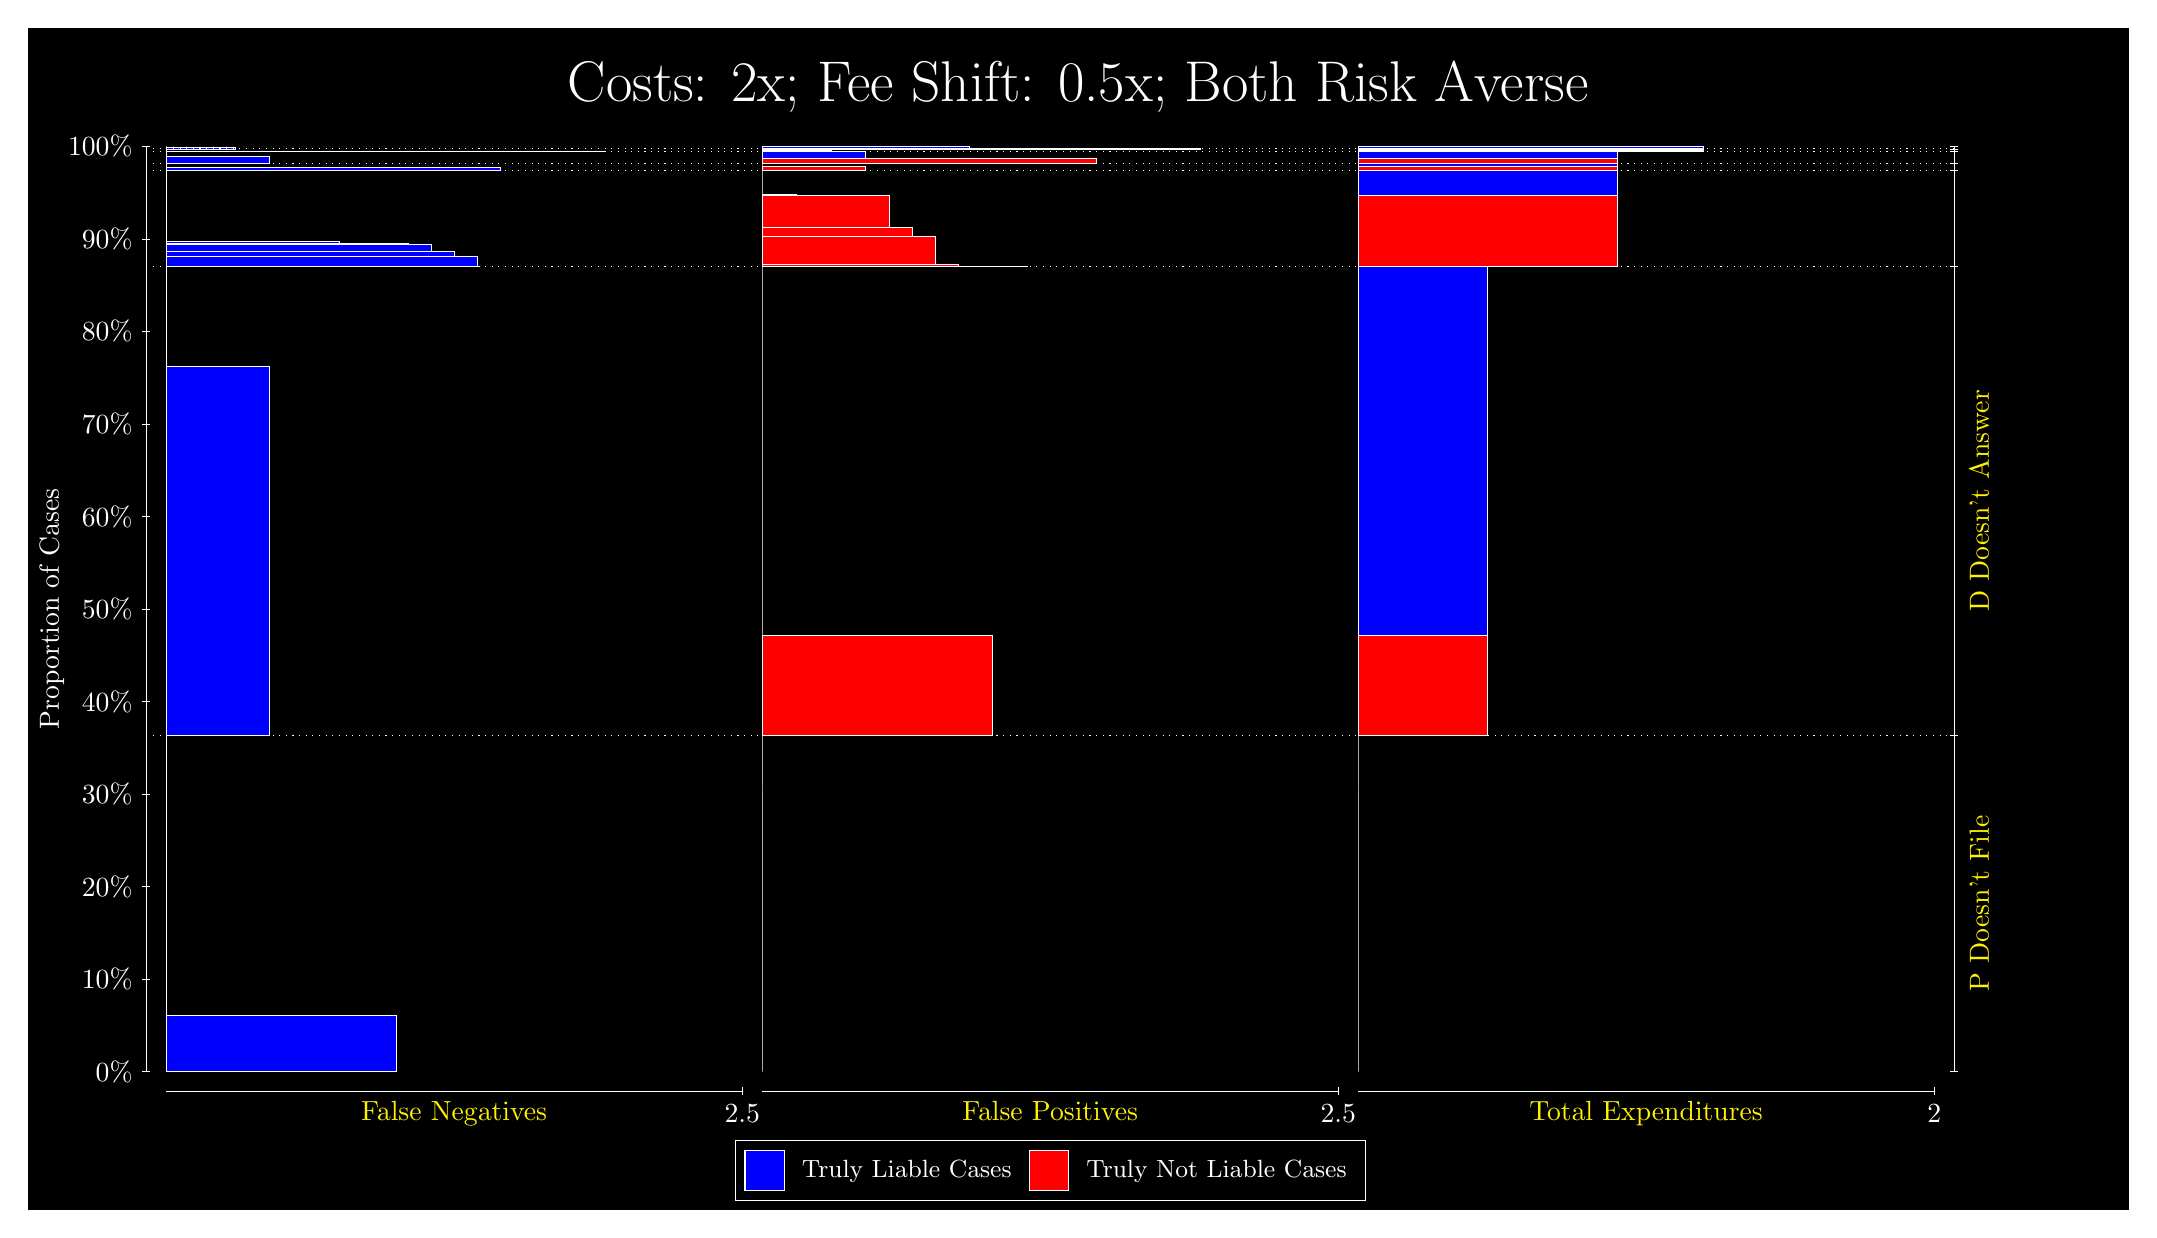
\begin{tikzpicture}
\draw[fill=black] (0,0) rectangle (26.667,15);
\draw[text=white] (0,13.5) rectangle (26.667,15) node[midway] {\huge Costs: 2x; Fee Shift: 0.5x; Both Risk Averse};
\draw[white, very thin] (1.5,1.75) -- (1.5,13.5);
\node[rotate=90, text=white, anchor=center] at (0.3, 7.625) {Proportion of Cases};
\draw[white, very thin] (1.45,1.75) -- (1.55,1.75);
\node[text=white, anchor=east] at (1.45, 1.75) {0\%};
\draw[white, very thin] (1.45,2.925) -- (1.55,2.925);
\node[text=white, anchor=east] at (1.45, 2.925) {10\%};
\draw[white, very thin] (1.45,4.1) -- (1.55,4.1);
\node[text=white, anchor=east] at (1.45, 4.1) {20\%};
\draw[white, very thin] (1.45,5.275) -- (1.55,5.275);
\node[text=white, anchor=east] at (1.45, 5.275) {30\%};
\draw[white, very thin] (1.45,6.45) -- (1.55,6.45);
\node[text=white, anchor=east] at (1.45, 6.45) {40\%};
\draw[white, very thin] (1.45,7.625) -- (1.55,7.625);
\node[text=white, anchor=east] at (1.45, 7.625) {50\%};
\draw[white, very thin] (1.45,8.8) -- (1.55,8.8);
\node[text=white, anchor=east] at (1.45, 8.8) {60\%};
\draw[white, very thin] (1.45,9.975) -- (1.55,9.975);
\node[text=white, anchor=east] at (1.45, 9.975) {70\%};
\draw[white, very thin] (1.45,11.15) -- (1.55,11.15);
\node[text=white, anchor=east] at (1.45, 11.15) {80\%};
\draw[white, very thin] (1.45,12.325) -- (1.55,12.325);
\node[text=white, anchor=east] at (1.45, 12.325) {90\%};
\draw[white, very thin] (1.45,13.5) -- (1.55,13.5);
\node[text=white, anchor=east] at (1.45, 13.5) {100\%};

\draw[white, very thin] (24.457,1.75) -- (24.457,13.5);
\draw[white, very thin] (24.407,1.75) -- (24.507,1.75);
\node[anchor=west] at (24.407, 1.75) {};
\draw[white, very thin] (24.407,6.0192) -- (24.507,6.0192);
\node[anchor=west] at (24.407, 6.0192) {};
\draw[white, very thin] (24.407,11.974) -- (24.507,11.974);
\node[anchor=west] at (24.407, 11.974) {};
\draw[white, very thin] (24.407,13.195) -- (24.507,13.195);
\node[anchor=west] at (24.407, 13.195) {};
\draw[white, very thin] (24.407,13.285) -- (24.507,13.285);
\node[anchor=west] at (24.407, 13.285) {};
\draw[white, very thin] (24.407,13.431) -- (24.507,13.431);
\node[anchor=west] at (24.407, 13.431) {};
\draw[white, very thin] (24.407,13.468) -- (24.507,13.468);
\node[anchor=west] at (24.407, 13.468) {};
\draw[white, very thin] (24.407,13.5) -- (24.507,13.5);
\node[anchor=west] at (24.407, 13.5) {};

\draw[white, very thin, fill=blue] (1.75,1.75) rectangle (4.6775,2.4615);
\draw[white, very thin, fill=red] (1.75,2.4615) rectangle (1.75,6.0192);
\draw[white, very thin, fill=blue] (1.75,6.0192) rectangle (3.0674,10.707);
\draw[white, very thin, fill=red] (1.75,10.707) rectangle (1.75,11.974);
\draw[white, very thin, fill=blue] (1.75,11.974) rectangle (5.7022,12.107);
\draw[white, very thin, fill=blue] (1.75,12.107) rectangle (5.4094,12.161);
\draw[white, very thin, fill=blue] (1.75,12.161) rectangle (5.1167,12.251);
\draw[white, very thin, fill=blue] (1.75,12.251) rectangle (4.8239,12.274);
\draw[white, very thin, fill=blue] (1.75,12.274) rectangle (4.5312,12.274);
\draw[white, very thin, fill=blue] (1.75,12.274) rectangle (3.9457,12.297);
\draw[white, very thin, fill=red] (1.75,12.297) rectangle (1.75,13.195);
\draw[white, very thin, fill=blue] (1.75,13.195) rectangle (5.9949,13.232);
\draw[white, very thin, fill=red] (1.75,13.232) rectangle (1.75,13.285);
\draw[white, very thin, fill=blue] (1.75,13.285) rectangle (3.0674,13.368);
\draw[white, very thin, fill=red] (1.75,13.368) rectangle (1.75,13.431);
\draw[white, very thin, fill=blue] (1.75,13.431) rectangle (7.3123,13.443);
\draw[white, very thin, fill=red] (1.75,13.443) rectangle (1.75,13.468);
\draw[white, very thin, fill=blue] (1.75,13.468) rectangle (2.6283,13.488);
\draw[white, very thin, fill=red] (1.75,13.488) rectangle (1.75,13.5);
\draw[white, very thin, fill=red] (9.3189,1.75) rectangle (9.3189,5.3077);
\draw[white, very thin, fill=blue] (9.3189,5.3077) rectangle (9.3189,6.0192);
\draw[white, very thin, fill=red] (9.3189,6.0192) rectangle (12.246,7.286);
\draw[white, very thin, fill=blue] (9.3189,7.286) rectangle (9.3189,11.974);
\draw[white, very thin, fill=red] (9.3189,11.974) rectangle (12.686,11.982);
\draw[white, very thin, fill=red] (9.3189,11.982) rectangle (12.1,11.982);
\draw[white, very thin, fill=red] (9.3189,11.982) rectangle (11.807,12.005);
\draw[white, very thin, fill=red] (9.3189,12.005) rectangle (11.515,12.36);
\draw[white, very thin, fill=red] (9.3189,12.36) rectangle (11.222,12.478);
\draw[white, very thin, fill=red] (9.3189,12.478) rectangle (10.929,12.872);
\draw[white, very thin, fill=blue] (9.3189,12.872) rectangle (9.758,12.894);
\draw[white, very thin, fill=blue] (9.3189,12.894) rectangle (9.3189,13.195);
\draw[white, very thin, fill=red] (9.3189,13.195) rectangle (10.636,13.247);
\draw[white, very thin, fill=blue] (9.3189,13.247) rectangle (9.3189,13.285);
\draw[white, very thin, fill=red] (9.3189,13.285) rectangle (13.564,13.348);
\draw[white, very thin, fill=blue] (9.3189,13.348) rectangle (10.636,13.431);
\draw[white, very thin, fill=red] (9.3189,13.431) rectangle (10.197,13.456);
\draw[white, very thin, fill=blue] (9.3189,13.456) rectangle (9.3189,13.468);
\draw[white, very thin, fill=red] (9.3189,13.468) rectangle (14.881,13.48);
\draw[white, very thin, fill=blue] (9.3189,13.48) rectangle (11.954,13.5);
\draw[white, very thin, fill=red] (16.888,1.75) rectangle (16.888,5.3077);
\draw[white, very thin, fill=blue] (16.888,5.3077) rectangle (16.888,6.0192);
\draw[white, very thin, fill=red] (16.888,6.0192) rectangle (18.534,7.286);
\draw[white, very thin, fill=blue] (16.888,7.286) rectangle (18.534,11.974);
\draw[white, very thin, fill=red] (16.888,11.974) rectangle (20.181,12.872);
\draw[white, very thin, fill=blue] (16.888,12.872) rectangle (20.181,13.195);
\draw[white, very thin, fill=red] (16.888,13.195) rectangle (20.181,13.247);
\draw[white, very thin, fill=blue] (16.888,13.247) rectangle (20.181,13.285);
\draw[white, very thin, fill=red] (16.888,13.285) rectangle (20.181,13.348);
\draw[white, very thin, fill=blue] (16.888,13.348) rectangle (20.181,13.431);
\draw[white, very thin, fill=red] (16.888,13.431) rectangle (21.279,13.456);
\draw[white, very thin, fill=blue] (16.888,13.456) rectangle (21.279,13.468);
\draw[white, very thin, fill=red] (16.888,13.468) rectangle (21.279,13.48);
\draw[white, very thin, fill=blue] (16.888,13.48) rectangle (21.279,13.5);
\draw[white, dotted] (1.5,6.0192) -- (24.457,6.0192);
\draw[white, dotted] (1.5,11.974) -- (24.457,11.974);
\draw[white, dotted] (1.5,13.195) -- (24.457,13.195);
\draw[white, dotted] (1.5,13.285) -- (24.457,13.285);
\draw[white, dotted] (1.5,13.431) -- (24.457,13.431);
\draw[white, dotted] (1.5,13.468) -- (24.457,13.468);
\draw[white, very thin] (1.75,1.5) -- (9.0689,1.5);
\node[text=yellow, anchor=north] at (5.4094, 1.5) {False Negatives};
\draw[white, very thin] (9.0689,1.45) -- (9.0689,1.55);
\node[text=white, anchor=north] at (9.0689, 1.45) {2.5};

\draw[white, very thin] (9.3189,1.5) -- (16.638,1.5);
\node[text=yellow, anchor=north] at (12.978, 1.5) {False Positives};
\draw[white, very thin] (16.638,1.45) -- (16.638,1.55);
\node[text=white, anchor=north] at (16.638, 1.45) {2.5};

\draw[white, very thin] (16.888,1.5) -- (24.207,1.5);
\node[text=yellow, anchor=north] at (20.547, 1.5) {Total Expenditures};
\draw[white, very thin] (24.207,1.45) -- (24.207,1.55);
\node[text=white, anchor=north] at (24.207, 1.45) {2};

\node[text=yellow, centered, rotate=90] at (24.777, 3.8846) {P Doesn't File};
\node[text=yellow, centered, rotate=90] at (24.777, 8.9964) {D Doesn't Answer};






\draw (12.978300999999998,1.5) node[draw=none] (baseCoordinate) {};
\begin{scope}[align=center]
        \matrix[scale=0.5, draw=white, below=0.5cm of baseCoordinate, nodes={draw}, column sep=0.1cm]{
            \node[rectangle, draw, minimum width=0.5cm, minimum height=0.5cm, fill=blue] {}; &
            \node[draw=none, font=\small, text=white] (B) {Truly Liable Cases}; &
            \node[rectangle, draw, minimum width=0.5cm, minimum height=0.5cm, fill=red] {}; &
            \node[draw=none, font=\small, text=white] (B) {Truly Not Liable Cases}; \\
            };
\end{scope}

\end{tikzpicture}
\end{document}